\section{Experiment}
\label{Sec:experiment}

We used two experimental testbeds to test the importance of \emph{split execution} for {\sf mxm} operation. Experiments were performed on a quad-core Intel Xeon CPU E5-2637 v2 @ 3.50GHz with 256 GB RAM running Ubuntu 14.04.1, and an NVIDIA K40c GPU with 12 GB RAM.

\begin{table}[htb]
	\hrule
	\caption{Experimental setup used for benchmarking.}
	\label{Tab:testbed}
	\begin{center}
	\begin{tabular}{|c|c|c|} \hline
		Vendor & Intel & Nvidia \\ \hline
		Family & Xeon & Tesla GPU \\
		Device & E5-2637 v2 & K40c \\
		Codename & Sandy Bridge & Kepler GK110 \\
		Memory & 256 GB & 12 GB \\
		OS & Ubuntu 14.04.1 & Ubuntu 14.04.1 \\
		Compiler & Intel C++ v17.0.4 & nvcc v8.0.44 \\
		 & Intel OpenMP v5.0 & g++ v4.9.4 \\
		Library & Intel MKL 2017.4.196 & cuSPARSE v8.0 \\ \hline
	\end{tabular}
	\end{center}
	\hrule
\end{table}

\begin{table}[htb]
	\hrule
	\caption{Description of datasets used for benchmarking. Flops refers to the number of floating-point computations required to square the matrix by itself. Two copies of the matrix are kept in memory for sake of benchmarking.}
	\label{Tab:testset}
	\begin{center}
		\begin{tabular}{|c|c|c|c|c|} \hline
			Dataset & Rows & Nonzeros & Flops & Symmetric\\ \hline
			Epidemiology & 526k & 2.1M & 16.8M & no \\
			Wind Tunnel & 218k & 11.6M & 1.3B & yes \\
			Protein & 36k & 4.3M & 1.1B & yes\\
			Sphere & 83k & 6.0M & 0.9B & yes\\
			Hood & 221k & 10.8M & 1.1B & yes \\
			Webbase & 1.0M & 3.1M & 139M & no \\ \hline
		\end{tabular}
	\end{center}
	\hrule
\end{table}

\begin{figure}
	\centering
	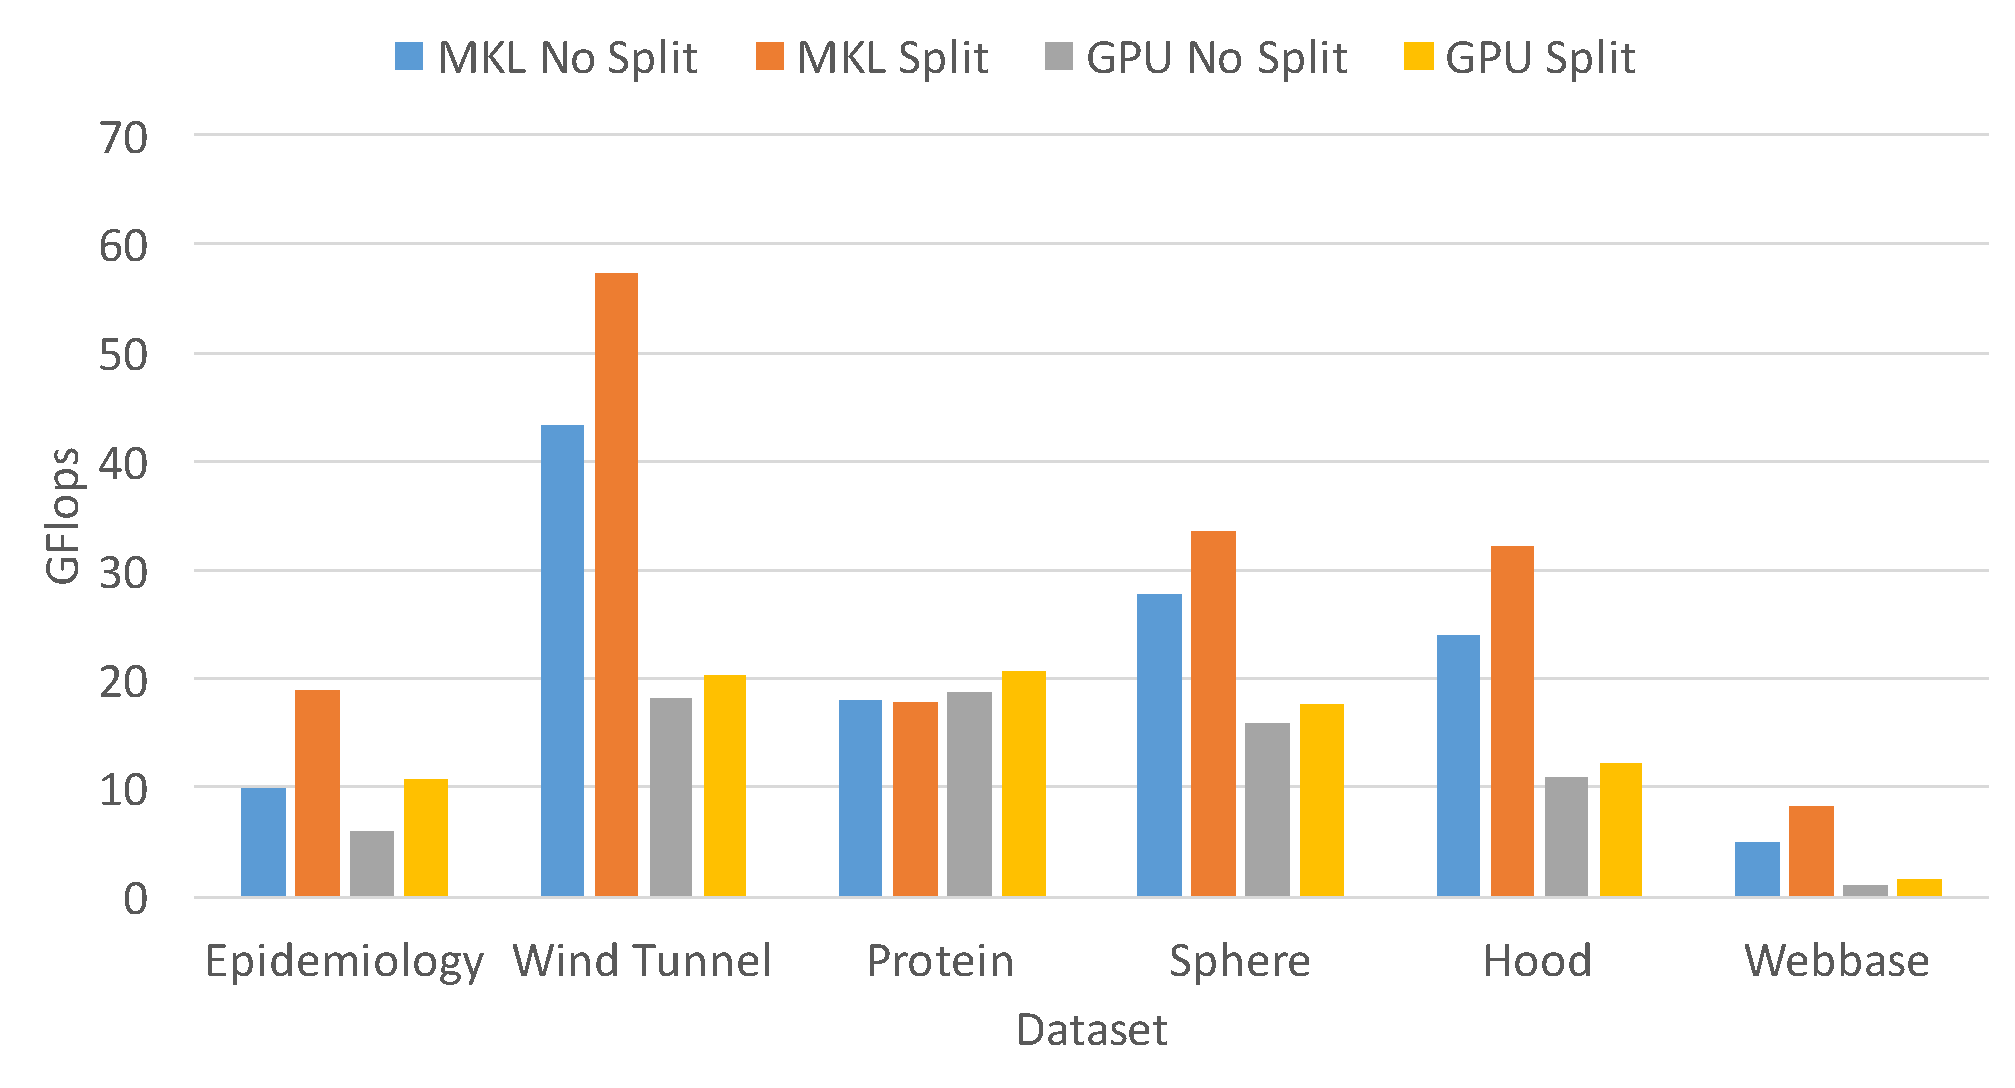
\includegraphics[width=.9\linewidth]{gflops.pdf}
	\caption{Comparison of {\sf mxm} runtime with and without split execution for two experimental setups.}
	\label{fig:gflops}
\end{figure}
